\input{../YKY-preamble.tex}
% \usepackage[no-math]{fontspec}
% \setmainfont[BoldFont=Alibaba_Sans_Regular.otf,ItalicFont=Alibaba_Sans_Light_Italic.otf]{Alibaba_Sans_Light.otf}

\usepackage[backend=biber]{biblatex}
\bibliography{../AGI-book}

\usepackage[active,tightpage]{preview}		% for continuous page(s)
\renewcommand{\PreviewBorder}{0.5cm}
\renewcommand{\thempfootnote}{\arabic{mpfootnote}}

\usepackage[absolute,overlay]{textpos}		% for page number on upper left corner
\usepackage{wrapfig}						% wrap text around figure

\usepackage{color}
% \usepackage{mathtools}
\usepackage[hyperfootnotes=false]{hyperref}

% \usepackage[backend=biber,style=numeric]{biblatex}
% \bibliography{../AGI-book}
% \renewcommand*{\bibfont}{\footnotesize}

\usetikzlibrary{shapes}
% \usepackage[export]{adjustbox}	% ??
\usepackage{verbatim} % for comments
% \usepackage{newtxtext,newtxmath}	% Times New Roman font

% \titleformat{\subsection}[hang]{\bfseries\large\color{blue}}{}{0pt}{} 
% \numberwithin{equation}{subsection}

\newcommand{\underdash}[1]{%
	\tikz[baseline=(toUnderline.base)]{
		\node[inner sep=1pt,outer sep=10pt] (toUnderline) {#1};
		\draw[dashed] ([yshift=-0pt]toUnderline.south west) -- ([yshift=-0pt]toUnderline.south east);
	}%
}%

\newcommand\reduline{\bgroup\markoverwith{\textcolor{red}{\rule[-0.5ex]{2pt}{0.4pt}}}\ULon}

%\DeclareSymbolFont{symbolsC}{U}{txsyc}{m}{n}
%\DeclareMathSymbol{\strictif}{\mathrel}{symbolsC}{74}
%\DeclareSymbolFont{AMSb}{U}{msb}{m}{n}
%\DeclareSymbolFontAlphabet{\mathbb}{AMSb}
%\setmathfont{lmroman17-regular.otf}
\DeclareMathOperator*{\argmin}{arg\,min}
\DeclareMathOperator*{\argmax}{arg\,max}

% \usepackage[most]{tcolorbox}
%\tcbset{on line, 
%	boxsep=4pt, left=0pt,right=0pt,top=0pt,bottom=0pt,
%	colframe=red,colback=pink,
%	highlight math style={enhanced}
%}
%\newcommand{\atom}{\vcenter{\hbox{\tcbox{....}}}}

\let\oldtextbf\textbf
\renewcommand{\textbf}[1]{\textcolor{blue}{\oldtextbf{#1}}}

\newcommand{\logic}[1]{{\color{violet}{\textit{#1}}}}
\newcommand{\underconst}{\includegraphics[scale=0.5]{../2020/UnderConst.png}}
\newcommand{\KBsymbol}{\vcenter{\hbox{\includegraphics[scale=1]{../KB-symbol.png}}}}
\newcommand{\token}{\vcenter{\hbox{\includegraphics[scale=1]{token.png}}}}
\newcommand{\proposition}{\vcenter{\hbox{\includegraphics[scale=0.8]{proposition.png}}}}

\begin{document}

\begin{preview}

\title{\vspace{-1.5cm} \bfseries\color{blue}{\LARGE Measuring the ``size'' of hypothesis spaces over $\mathbb{R}$ from the perspective of No Free Lunch}}

\author{Yan King Yin} % Your name
% \date{\vspace{-2cm}} % Date, can be changed to a custom date

\maketitle

\setcounter{section}{-1}
\newcounter{mypage}
\setcounter{mypage}{0}

% (1) Circled page number on upper left corner
\begin{textblock*}{5cm}(2.1cm,2.3cm) % {block width} (coords) 
{\color{red}{\large \textcircled{\small \themypage}}}
\addtocounter{mypage}{1}
\end{textblock*}

\begin{minipage}{\textwidth}
\setlength{\parskip}{0.4\baselineskip}

\section{Motivating example}

We want to learn, ie, use gradient descent of a neural network to approximate, a symmetric function $y = \hat{f}(\vec{x})$ satisfying the condition $\hat{f}(x_1, ... x_n) = \hat{f}( \sigma \cdot \{x_1, ... x_n\} )$ where $\sigma \in \mathfrak{S}_n$ is a permutation.  The \textbf{input space} is $X = \mathbb{R}^n = n$-dimensional hypercube:
\begin{equation}
\vcenter{\hbox{\includegraphics[scale=0.7]{cube-corner.png}}}
\end{equation}
Permutation symmetry implies that only one corner of the hypercube need be considered, this is the \textbf{fundamental domain}.  The \textbf{volume} of this domain over the entire hypercube shrinks exponentially as $n$ grows, so it appears that this symmetry is very significant for efficiency consideration.  We want to quantify the notion of this efficiency.

\section{Finding the right space setting}

We want to compare the \textbf{hypothesis spaces} $A$ and $B$:
\begin{itemize}
	\item $A$ = unconstrained, fully-connected neural network with $L$ layers and $N$ total weights.  The parameter space $A = \Theta_A = \mathbb{R}^N$.
	\item $B$ = symmetric neural network with a special structure but nonetheless its parameter space is also of the form $B = \Theta_B = \mathbb{R}^M$.
\end{itemize}

My first idea is to embed the space $B$ into space $A$.  This will lead to ``unwieldy'' elements of $B$ trying to approximate $A$, for example, consider if $A$'s activation function is sigmoid but $B$'s activation function is RELU.
\begin{equation}
\vcenter{\hbox{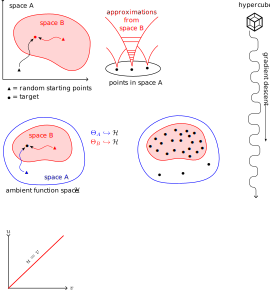
\includegraphics[scale=0.7]{no-free-lunch.png}}}
\end{equation}
But the general idea is: If solutions are only found in space $B$, then limiting our search within $B$ will lead to faster convergence as there is no need to waste time ``wandering'' in space $A$.

A better idea which is much more convenient is to consider $A$ and $B$ as both embedded in an ambient \textbf{function space} $\mathcal{H}$ that is ``fine'' enough to contain all points of $A$ and $B$:
\begin{equation}
\vcenter{\hbox{\includegraphics[scale=0.7]{no-free-lunch-2.png}}} \qquad
\begin{aligned}
& \text{Embeddings:} \\
& {\color{blue}\Theta_A \hookrightarrow} \; \mathcal{H} \\
& {\color{red}\Theta_B \hookrightarrow} \; \mathcal{H} 
\end{aligned}
\end{equation}

\section{Measure roughness of landscape?}

My second idea is to measure the ``roughness'' of the landscapes $A$ and $B$ in the function space $\mathcal{H}$.  The objective function is usually of the form
\begin{equation}
\text{loss} = \sum_i d( f(x_i; \Theta) , y_i ) + \text{Reg}(f)
\end{equation}
where $d$ is some distance metric and Reg is a regularization function.

\begin{wrapfigure}{r}{4cm}
	\centering
	\stepcounter{equation}
	\begin{equation}
	\vcenter{\hbox{\includegraphics[scale=0.75]{gradient-descent-from-hypercube.png}}}
	\tag{\theequation}
	\label{Fig-gradient-descent}
	\end{equation}
	\vspace{-2cm}
\end{wrapfigure}
The models in $A$ or $B$ live in the parameter spaces $\Theta_A$ or $\Theta_B$ and both are embedded into the space $\mathcal{H}$.  However the \textbf{paths} of gradient descent in $A$ or $B$ could still be different, so we have to be cautious about that.

In low-dimension space, we imagine being ``trapped'' in some kind of pit, so we may want to measure the roughness of the landscape by ``undulations'' of gradients.  But our next consideration suggests that this may not be a very effective measurement...

% For some reason I concluded that roughness of landscape is of secondary importance, why?

\section{Gradient descent in high-dimension space}

It may be helpful to visualize gradient descent in high-dimension space with Fig.(\ref{Fig-gradient-descent}).  Imagine the hypercube as having millions of vertices (as the number of weights).  The ``landscape'' is a surface sitting ``over'' the hypercube but we visualize it downwards.

It is very ``easy'' for gradient descent to find a way ``down'' because there are so many dimensions to choose from.

Also, a ``local minimum'' is very rare as it requires millions of gradients to be pointing ``up'' at the same spot.  In a model with a massive number of weights (as in the case of current LLMs), for all practical purposes, a local minimum is just as good as an acceptable solution.  In this sense, \textit{the phenomenon of ``getting stuck in local minima'' disappears}.

\section{The ``symmetric'' parameter space}

The following figure may help visualize the parameter space of our \textbf{symmetric} motivating example (but not for the AGI problem).

In our example, $\Theta_A = (u, v)$ but $\Theta_B$ is just the diagonal space $\langle u = v \rangle$.  The case with 3 parameters, of which 2 are equal, is shown on the right:
\begin{equation}
\vcenter{\hbox{\includegraphics[scale=0.7]{symmetric-space.png}}}
\end{equation}
In general, multiple dimensions can collapse to one, when the weights are shared (equal).

\section{Distribution of solution ``attractors''}

I find the most helpful way to visualize the AGI landscape is to imagine solution \textbf{attractors} to be more \textit{densely} populated in the more-structured space $B$.

The following is a diagram I made up using a Python script and Matplotlib with randomly generated plots.  One can imagine ''attractors'' for \textbf{gradient descent} that are distributed over the hypothesis space that lead to solutions (AGIs).  I made the distribution of attractors in space $B$ \textbf{denser} than in space $A$.  So if an algorithm randomly starts to search, it will have a better chance of success to start within space $B$.  The ``distances'' traveled by gradient descent are also different for $A$ and $B$ because their parameter spaces are different.

\begin{equation}
\vcenter{\hbox{\includegraphics[scale=1]{AGI-attractors.png}}}
\end{equation}
Perhaps the most crucial thing we want to prove, or at least find indirect evidence for, is whether solution attractors are \textbf{sparser} in space $A$ than $B$.  This is obviously a \textbf{problem-specific} question.  In some cases, such as the learning of symmetric functions, we know \textit{a priori} that solutions \textit{exclusively} lie in space $B$.  But the issue is very hard to analyze for AGI.


% 问题 1: 究竟是有很多个解分布在不同区域,还是有一个比较大的单一连通的解区域?  似乎是前者,因为有很多不同的初始 directions 是可以得到 non-identical but effectively equivalent 的解。 

% 问题 2: 是否存在很多 local minima 陷阱? 其实此问题并不影响我们研究的问题。 而且答案似乎是否定的。



\end{minipage}
\end{preview}

\begin{preview}
\begin{textblock*}{5cm}(2.1cm,2.3cm) % {block width} (coords) 
	{\color{red}{\large \textcircled{\small \themypage}}}
	\addtocounter{mypage}{1}
\end{textblock*}

\begin{minipage}{\textwidth}
	\setlength{\parskip}{0.4\baselineskip}

\section{This}

\begin{itemize}
	\item Here
\end{itemize}

\end{minipage}
\end{preview}

\begin{preview}
\begin{textblock*}{5cm}(2.1cm,2.3cm) % {block width} (coords) 
{\color{red}{\large \textcircled{\small \themypage}}}
\addtocounter{mypage}{1}
\end{textblock*}

\begin{minipage}{\textwidth}
\setlength{\parskip}{0.4\baselineskip}

\section{This}

\begin{itemize}
	\item Here
\end{itemize}

\end{minipage}
\end{preview}

\begin{preview}
\begin{textblock*}{5cm}(2.1cm,2.3cm) % {block width} (coords) 
	{\color{red}{\large \textcircled{\small \themypage}}}
	\addtocounter{mypage}{1}
\end{textblock*}

\begin{minipage}{\textwidth}
	\setlength{\parskip}{0.4\baselineskip}

\section{This}

\begin{itemize}
	\item Here
\end{itemize}

\end{minipage}
\end{preview}

\end{document}
